\documentclass[border=3pt,10pt]{standalone}
\usepackage{times}
\usepackage{amsmath, amsfonts, bm}
\usepackage{tikz}
\usetikzlibrary{arrows.meta}

\begin{document}
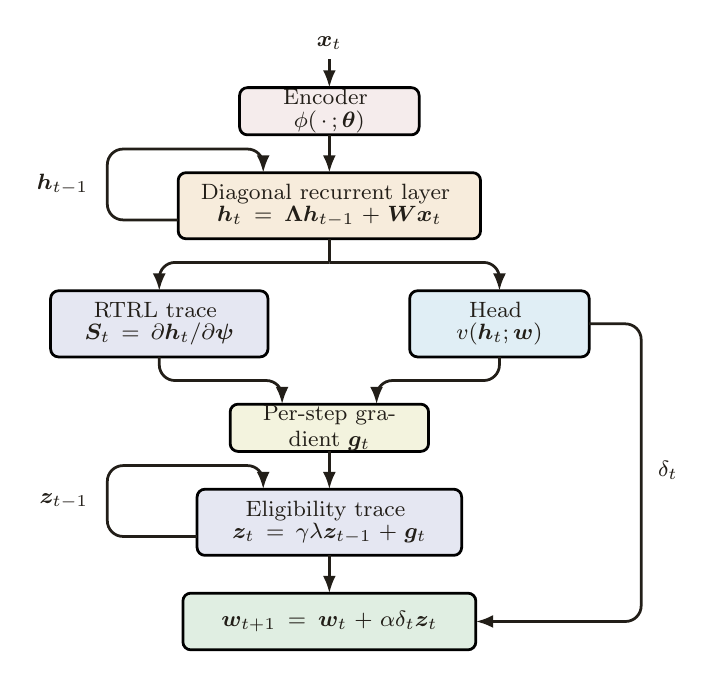
\begin{tikzpicture}[x=0.6cm, y=0.6cm, font=\footnotesize]

\definecolor{encoder_color}{RGB}{245,236,236}
\definecolor{rec_color}{RGB}{247,236,220}
\definecolor{head_color}{RGB}{224,238,245}
\definecolor{trace_color}{RGB}{229,231,242}
\definecolor{grad_color}{RGB}{243,243,222}
\definecolor{update_color}{RGB}{224,238,226}
\definecolor{blocktext}{RGB}{34,30,24}

\tikzset{
  wire/.style={line width=0.035cm, draw=blocktext},
  ar/.style={-{Latex[length=2.2mm]}, line width=0.035cm, draw=blocktext, rounded corners=0.2cm},
  lab/.style={text=blocktext, align=center},
}

\newcommand{\blk}[6]{%
  \draw[line width=0.035cm, fill=#5, rounded corners=0.1cm]
    (#1-#3, #2+#4) -- (#1+#3, #2+#4) -- (#1+#3, #2-#4) -- (#1-#3, #2-#4) -- cycle;
  \node[text width=1.2*#3 cm, align=center, text=blocktext] at (#1, #2) {#6};
}

\blk{0}{9.2}{1.9}{0.5}{encoder_color}{Encoder \vspace{-0.05cm} \linebreak $\phi(\,\cdot\,;\bm{\theta})$}
\blk{0}{7.2}{3.2}{0.7}{rec_color}{Diagonal recurrent layer \vspace{-0.05cm} \linebreak $\bm{h}_t = \bm{\Lambda}\bm{h}_{t-1} + \bm{W}\bm{x}_t$}
\blk{-3.6}{4.7}{2.3}{0.7}{trace_color}{RTRL trace \vspace{-0.05cm} \linebreak $\bm{S}_t = \partial\bm{h}_t / \partial\bm{\psi}$}
\blk{3.6}{4.7}{1.9}{0.7}{head_color}{Head \vspace{-0.05cm} \linebreak $v(\bm{h}_t;\bm{w})$}
\blk{0}{2.5}{2.1}{0.5}{grad_color}{Per-step gradient $\bm{g}_t$}
\blk{0}{0.5}{2.8}{0.7}{trace_color}{Eligibility trace \vspace{-0.05cm} \linebreak $\bm{z}_t = \gamma\lambda\bm{z}_{t-1} + \bm{g}_t$}
\blk{0}{-1.6}{3.1}{0.6}{update_color}{$\bm{w}_{t+1} = \bm{w}_t + \alpha\delta_t\bm{z}_t$}

\node[lab, anchor=south] at (0, 10.3) {$\bm{x}_t$};

\draw[ar] (0, 10.3) -- (0, 9.7);
\draw[ar] (0, 8.7) -- (0, 7.9);
\draw[wire] (0, 6.5) -- (0, 6.0);
\draw[ar] (0, 6.0) -- (-3.6, 6.0) -- (-3.6, 5.4);
\draw[ar] (0, 6.0) -- (3.6, 6.0) -- (3.6, 5.4);
\draw[ar] (-3.6, 4.0) -- (-3.6, 3.5) -- (-1.0, 3.5) -- (-1.0, 3.0);
\draw[ar] (3.6, 4.0) -- (3.6, 3.5) -- (1.0, 3.5) -- (1.0, 3.0);
\draw[ar] (0, 2.0) -- (0, 1.2);
\draw[ar] (0, -0.2) -- (0, -1.0);

\draw[ar] (5.5, 4.7) -- (6.6, 4.7) -- (6.6, -1.6) -- (3.1, -1.6);
\node[lab, anchor=west] at (6.75, 1.6) {$\delta_t$};

\draw[ar] (-3.2, 6.9) -- (-4.7, 6.9) -- (-4.7, 8.4) -- (-1.4, 8.4) -- (-1.4, 7.9);
\node[lab, anchor=east] at (-4.9, 7.65) {$\bm{h}_{t-1}$};

\draw[ar] (-2.8, 0.2) -- (-4.7, 0.2) -- (-4.7, 1.7) -- (-1.4, 1.7) -- (-1.4, 1.2);
\node[lab, anchor=east] at (-4.9, 0.95) {$\bm{z}_{t-1}$};

\end{tikzpicture}
\end{document}
